% NVIDIA Ecosystem LaTeX Book
% Compile with: pdflatex --shell-escape filename.tex
\documentclass[12pt,a4paper,oneside]{book}

% ==================== PACKAGES ====================
\usepackage[utf8]{inputenc}
\usepackage[T1]{fontenc}
\usepackage{lmodern}
\usepackage[margin=1in]{geometry}
\usepackage{xcolor}
\usepackage{graphicx}
\usepackage{tikz}
\usetikzlibrary{shapes.geometric, arrows.meta, positioning, shadows, backgrounds, fit, calc}
\usepackage{tcolorbox}
\tcbuselibrary{skins,breakable}
\usepackage{fancyhdr}
\usepackage{hyperref}
\usepackage{titlesec}
\usepackage{enumitem}
\usepackage{booktabs}
\usepackage{tabularx}
\usepackage{longtable}
\usepackage{array}
\usepackage{float}
\usepackage{caption}
\usepackage{subcaption}
\usepackage{listings}
\usepackage{amsmath}
\usepackage{amssymb}

% ==================== COLOR DEFINITIONS ====================
\definecolor{nvidiagreen}{RGB}{118,185,0}      % #76b900
\definecolor{nvidiablack}{RGB}{0,0,0}          % #000000
\definecolor{nvidiadarkgray}{RGB}{25,25,25}
\definecolor{nvidialightgray}{RGB}{200,200,200}
\definecolor{nvidiawhite}{RGB}{255,255,255}
\definecolor{nvidiablue}{RGB}{0,120,212}
\definecolor{accentorange}{RGB}{255,140,0}

% ==================== HYPERREF SETUP ====================
\hypersetup{
    colorlinks=true,
    linkcolor=nvidiagreen,
    filecolor=nvidiagreen,
    urlcolor=nvidiablue,
    citecolor=nvidiagreen,
    pdftitle={NVIDIA Ecosystem Guide},
    pdfauthor={Yash Kavaiya - Easy AI Labs},
    pdfsubject={NVIDIA AI Infrastructure},
    pdfkeywords={NVIDIA, AI, GPU, Deep Learning}
}

% ==================== TITLE FORMATTING ====================
\titleformat{\chapter}[display]
{\normalfont\huge\bfseries\color{nvidiagreen}}
{\chaptertitlename\ \thechapter}{20pt}{\Huge\color{nvidiagreen}}

\titleformat{\section}
{\normalfont\Large\bfseries\color{nvidiagreen}}
{\thesection}{1em}{}

\titleformat{\subsection}
{\normalfont\large\bfseries\color{nvidiablue}}
{\thesubsection}{1em}{}

% ==================== HEADER AND FOOTER ====================
\pagestyle{fancy}
\fancyhf{}
\fancyhead[L]{\textcolor{nvidiagreen}{\leftmark}}
\fancyhead[R]{\textcolor{nvidiagreen}{\thepage}}
\fancyfoot[L]{\small\href{https://easy-ai-labs.lovable.app/}{\textcolor{nvidiablue}{Easy AI Labs}}}
\fancyfoot[C]{\small\href{https://www.linkedin.com/in/yashkavaiya}{\textcolor{nvidiablue}{Yash Kavaiya}}}
\fancyfoot[R]{\small\href{https://www.linkedin.com/company/genai-guru}{\textcolor{nvidiablue}{Gen AI Guru}}}
\renewcommand{\headrulewidth}{0.5pt}
\renewcommand{\footrulewidth}{0.5pt}
\renewcommand{\headrule}{\hbox to\headwidth{\color{nvidiagreen}\leaders\hrule height \headrulewidth\hfill}}
\renewcommand{\footrule}{\hbox to\headwidth{\color{nvidiagreen}\leaders\hrule height \footrulewidth\hfill}}

% ==================== CUSTOM BOXES ====================
\newtcolorbox{nvidiabox}[1][]{
    colback=nvidiablack!5,
    colframe=nvidiagreen,
    fonttitle=\bfseries\color{nvidiawhite},
    title=#1,
    enhanced,
    attach boxed title to top left={yshift=-2mm,xshift=5mm},
    boxed title style={colback=nvidiagreen},
    sharp corners,
    breakable
}

\newtcolorbox{keypoint}{
    colback=nvidiagreen!10,
    colframe=nvidiagreen,
    fonttitle=\bfseries,
    title=Key Point,
    enhanced,
    left=5pt,
    right=5pt,
    breakable
}

% ==================== LISTINGS SETUP ====================
\lstset{
    basicstyle=\ttfamily\small,
    backgroundcolor=\color{nvidiablack!5},
    frame=single,
    rulecolor=\color{nvidiagreen},
    numbers=left,
    numberstyle=\tiny\color{nvidialightgray},
    keywordstyle=\color{nvidiagreen}\bfseries,
    commentstyle=\color{nvidialightgray}\itshape,
    stringstyle=\color{nvidiablue},
    breaklines=true,
    showstringspaces=false
}

% ==================== DOCUMENT BEGIN ====================
\begin{document}

% ==================== TITLE PAGE ====================
\begin{titlepage}
    \begin{tikzpicture}[remember picture,overlay]
        % Black background
        \fill[nvidiablack] (current page.south west) rectangle (current page.north east);
        
        % NVIDIA green accent bars
        \fill[nvidiagreen] (current page.north west) rectangle ([yshift=-2cm]current page.north east);
        \fill[nvidiagreen] ([yshift=2cm]current page.south west) rectangle (current page.south east);
        
        % Title
        \node[text=nvidiawhite,font=\fontsize{48}{58}\selectfont\bfseries] at ([yshift=3cm]current page.center) {NVIDIA};
        \node[text=nvidiagreen,font=\fontsize{36}{44}\selectfont\bfseries] at ([yshift=0.5cm]current page.center) {Ecosystem Guide};
        \node[text=nvidiawhite,font=\fontsize{20}{24}\selectfont] at ([yshift=-2cm]current page.center) {Complete AI Infrastructure Overview};
        
        % Authors
        \node[text=nvidiawhite,font=\fontsize{16}{20}\selectfont] at ([yshift=-5cm]current page.center) {By Yash Kavaiya};
        \node[text=nvidiagreen,font=\fontsize{14}{18}\selectfont] at ([yshift=-6cm]current page.center) {Easy AI Labs | Gen AI Guru};
        
        % Date
        \node[text=nvidialightgray,font=\fontsize{12}{16}\selectfont] at ([yshift=-8cm]current page.center) {\today};
    \end{tikzpicture}
\end{titlepage}

% ==================== TABLE OF CONTENTS ====================
\tableofcontents
\newpage

% ==================== CHAPTER 1: INTRODUCTION ====================
\chapter{Introduction to NVIDIA Ecosystem}

\section{Overview}

The NVIDIA ecosystem represents far more than GPU manufacturing. It encompasses a comprehensive suite of technologies, services, and tools specifically designed for machine learning, generative AI, and large language models. This ecosystem has positioned NVIDIA as a critical player in the generative AI revolution.

\begin{keypoint}
NVIDIA's success stems not just from hardware excellence, but from building a complete ecosystem that integrates seamlessly from silicon to software, enabling developers to maximize their AI investments.
\end{keypoint}

\section{Historical Evolution}

\begin{nvidiabox}[NVIDIA Timeline]
Understanding NVIDIA's journey helps contextualize their current dominance in AI infrastructure.
\end{nvidiabox}

\begin{table}[H]
\centering
\caption{NVIDIA Historical Milestones}
\begin{tabularx}{\textwidth}{>{\bfseries}l X}
\toprule
\textcolor{nvidiagreen}{Year} & \textcolor{nvidiagreen}{Milestone} \\
\midrule
1993 & Foundation of NVIDIA Corporation \\
1995 & Introduction of first graphics card \\
1999 & Launch of GeForce 256 - coined term "GPU" (Graphics Processing Unit) \\
2000s & Development of CUDA framework for general-purpose GPU computing \\
2010 & Establishment in parallel computing space \\
2020+ & Dominant player in AI and machine learning infrastructure \\
\bottomrule
\end{tabularx}
\label{tab:timeline}
\end{table}

\subsection{The Gaming Foundation (1990s-2000s)}

NVIDIA's initial success came through the gaming industry. The GeForce 256, launched in 1999, revolutionized 3D gaming and established NVIDIA's market dominance for years. This graphics card introduced the concept of the GPU as a dedicated parallel processing unit.

\subsection{The CUDA Revolution (2006-2010)}

The introduction of CUDA (Compute Unified Device Architecture) marked a pivotal shift. NVIDIA recognized that GPUs' parallel processing capabilities could extend far beyond graphics rendering, opening doors to scientific computing, data analysis, and eventually, AI.

\subsection{The AI Era (2010-Present)}

By 2020, NVIDIA had become the dominant force in AI infrastructure. Their GPUs became essential for training deep learning models, and their ecosystem expanded to include specialized frameworks, libraries, and deployment tools.

% ==================== NVIDIA ECOSYSTEM DIAGRAM ====================
\newpage
\section{NVIDIA Ecosystem Architecture}

\begin{figure}[H]
\centering
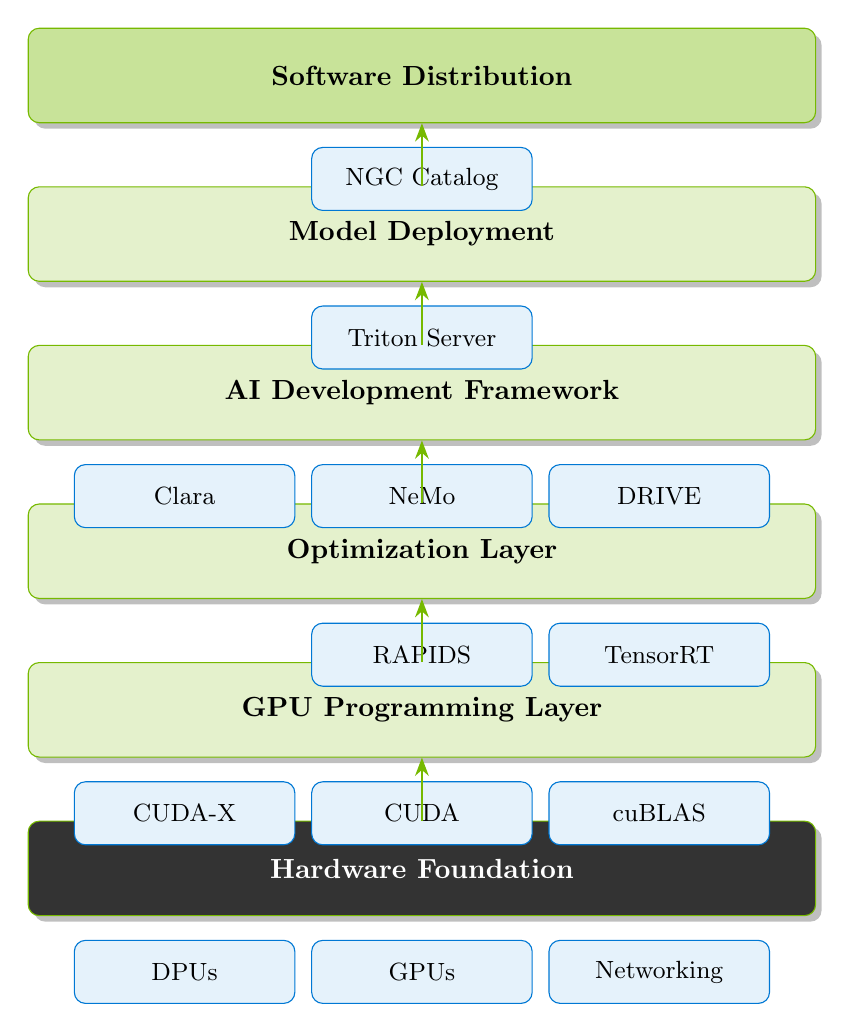
\begin{tikzpicture}[
    node distance=0.8cm,
    layer/.style={rectangle, rounded corners, minimum width=10cm, minimum height=1.2cm, text centered, draw=nvidiagreen, fill=nvidiagreen!20, font=\bfseries, drop shadow},
    component/.style={rectangle, rounded corners, minimum width=2.8cm, minimum height=0.8cm, text centered, draw=nvidiablue, fill=nvidiablue!10, font=\small},
    arrow/.style={-Stealth, thick, color=nvidiagreen}
]

% Layers from bottom to top
\node[layer, fill=nvidiablack!80, text=nvidiawhite] (hardware) {Hardware Foundation};
\node[layer, above=of hardware] (programming) {GPU Programming Layer};
\node[layer, above=of programming] (optimization) {Optimization Layer};
\node[layer, above=of optimization] (framework) {AI Development Framework};
\node[layer, above=of framework] (deployment) {Model Deployment};
\node[layer, above=of deployment, fill=nvidiagreen!40] (distribution) {Software Distribution};

% Components for each layer
\node[component, below=0.3cm of hardware] (gpu) {GPUs};
\node[component, left=0.2cm of gpu] (dpu) {DPUs};
\node[component, right=0.2cm of gpu] (network) {Networking};

\node[component, below=0.3cm of programming] (cuda) {CUDA};
\node[component, left=0.2cm of cuda] (cudax) {CUDA-X};
\node[component, right=0.2cm of cuda] {cuBLAS};

\node[component, below=0.3cm of optimization] (rapids) {RAPIDS};
\node[component, right=0.2cm of rapids] (tensorrt) {TensorRT};

\node[component, below=0.3cm of framework] (nemo) {NeMo};
\node[component, left=0.2cm of nemo] (clara) {Clara};
\node[component, right=0.2cm of nemo] (drive) {DRIVE};

\node[component, below=0.3cm of deployment] (triton) {Triton Server};

\node[component, below=0.3cm of distribution] (ngc) {NGC Catalog};

% Arrows showing flow
\draw[arrow] (hardware) -- (programming);
\draw[arrow] (programming) -- (optimization);
\draw[arrow] (optimization) -- (framework);
\draw[arrow] (framework) -- (deployment);
\draw[arrow] (deployment) -- (distribution);

\end{tikzpicture}
\caption{NVIDIA AI Stack Architecture - Layer-by-Layer View}
\label{fig:ecosystem}
\end{figure}

% ==================== CHAPTER 2: LAYER BREAKDOWN ====================
\chapter{NVIDIA Stack: Layer-by-Layer Analysis}

\section{Layer 1: Hardware Foundation}

\begin{nvidiabox}[Core Infrastructure]
The foundation of NVIDIA's ecosystem rests on specialized hardware designed for parallel processing and AI workloads.
\end{nvidiabox}

\subsection{NVIDIA GPUs}

NVIDIA GPUs are purpose-built for massive parallel computation. Unlike CPUs that excel at sequential processing, GPUs contain thousands of smaller cores designed to handle multiple tasks simultaneously.

\begin{table}[H]
\centering
\caption{NVIDIA GPU Architectures for AI}
\begin{tabularx}{\textwidth}{l X l l}
\toprule
\textcolor{nvidiagreen}{\textbf{Architecture}} & \textcolor{nvidiagreen}{\textbf{Key Features}} & \textcolor{nvidiagreen}{\textbf{Year}} & \textcolor{nvidiagreen}{\textbf{Use Case}} \\
\midrule
Volta & First Tensor Cores & 2017 & Deep Learning Training \\
Turing & RT Cores + Tensor Cores & 2018 & AI + Graphics \\
Ampere & 3rd Gen Tensor Cores & 2020 & Large-scale AI \\
Hopper & Transformer Engine & 2022 & LLM Training \\
Blackwell & Next-gen AI acceleration & 2024 & Future AI Workloads \\
\bottomrule
\end{tabularx}
\label{tab:gpu-arch}
\end{table}

\subsection{Additional Hardware Components}

\begin{itemize}[leftmargin=*, itemsep=8pt]
    \item \textbf{DPUs (Data Processing Units):} Specialized processors for data center infrastructure tasks, offloading networking, security, and storage operations from CPUs
    \item \textbf{InfiniBand Networking:} High-bandwidth, low-latency networking fabric enabling efficient multi-GPU and multi-node communication
    \item \textbf{DGX Systems:} Integrated AI supercomputers combining GPUs, networking, and software in turnkey solutions
\end{itemize}

\section{Layer 2: GPU Programming Platform}

\subsection{CUDA: Compute Unified Device Architecture}

CUDA revolutionized GPU computing by making parallel processing accessible to developers through C/C++ extensions.

\begin{nvidiabox}[CUDA Core Capabilities]
\begin{itemize}[leftmargin=*, itemsep=5pt]
    \item Parallel thread execution across thousands of GPU cores
    \item Unified memory management between CPU and GPU
    \item Rich library ecosystem for specialized computations
    \item Cross-platform support (Windows, Linux, macOS)
    \item Integration with popular programming languages
\end{itemize}
\end{nvidiabox}

\subsection{CUDA-X Libraries}

CUDA-X represents a collection of specialized libraries built on CUDA for domain-specific acceleration:

\begin{table}[H]
\centering
\caption{Key CUDA-X Libraries}
\begin{tabularx}{\textwidth}{l X}
\toprule
\textcolor{nvidiagreen}{\textbf{Library}} & \textcolor{nvidiagreen}{\textbf{Purpose}} \\
\midrule
cuBLAS & Basic Linear Algebra Subprograms (matrix operations) \\
cuDNN & Deep Neural Networks (convolutions, activations) \\
cuSPARSE & Sparse matrix operations \\
cuFFT & Fast Fourier Transforms \\
Thrust & Parallel algorithms and data structures \\
TensorRT & Deep learning inference optimization \\
\bottomrule
\end{tabularx}
\label{tab:cudax}
\end{table}

\section{Layer 3: Optimization Layer}

\subsection{RAPIDS: Accelerated Data Science}

RAPIDS enables end-to-end data science workflows on GPUs, dramatically reducing processing time for data preparation and analysis.

\begin{figure}[H]
\centering
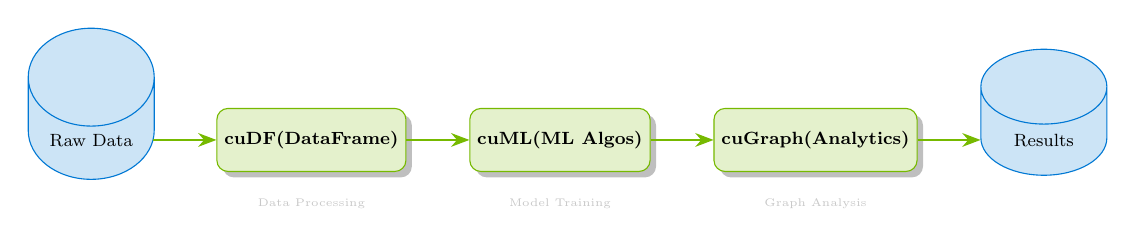
\begin{tikzpicture}[
    scale=0.8,            % <--- main global size control
    transform shape,      % scales nodes/text too
    node distance=1cm,
    block/.style={rectangle, rounded corners, minimum width=1.5cm, minimum height=1cm,
                  text centered, draw=nvidiagreen, fill=nvidiagreen!20,
                  font=\footnotesize\bfseries, drop shadow},
    data/.style={cylinder, shape border rotate=90, minimum height=2cm, minimum width=2cm,
                 draw=nvidiablue, fill=nvidiablue!20, font=\footnotesize},
    arrow/.style={-Stealth, thick, color=nvidiagreen}
]

\node[data] (rawdata) {Raw Data};
\node[block, right=of rawdata] (cudf) {cuDF\\(DataFrame)};
\node[block, right=of cudf] (cuml) {cuML\\(ML Algos)};
\node[block, right=of cuml] (cugraph) {cuGraph\\(Analytics)};
\node[data, right=of cugraph] (results) {Results};

\draw[arrow] (rawdata) -- (cudf);
\draw[arrow] (cudf) -- (cuml);
\draw[arrow] (cuml) -- (cugraph);
\draw[arrow] (cugraph) -- (results);

\node[below=0.3cm of cudf, font=\tiny, text=nvidialightgray] {Data Processing};
\node[below=0.3cm of cuml, font=\tiny, text=nvidialightgray] {Model Training};
\node[below=0.3cm of cugraph, font=\tiny, text=nvidialightgray] {Graph Analysis};

\end{tikzpicture}
\caption{RAPIDS data science pipeline}
\label{fig:rapids}
\end{figure}

\caption{RAPIDS Data Science Pipeline}
\label{fig:rapids}
\end{figure}

\textbf{RAPIDS Components:}
\begin{itemize}[leftmargin=*, itemsep=5pt]
    \item \textbf{cuDF:} GPU-accelerated DataFrame library (pandas-like API)
    \item \textbf{cuML:} Machine learning algorithms on GPU (scikit-learn-like API)
    \item \textbf{cuGraph:} Graph analytics acceleration
    \item \textbf{cuSpatial:} Geospatial data processing
\end{itemize}

\subsection{TensorRT: Inference Optimization}

TensorRT optimizes trained neural networks for production deployment, achieving significantly faster inference with lower latency.

\begin{keypoint}
TensorRT can deliver up to 40x faster inference compared to CPU-only deployment, with precision calibration (FP32, FP16, INT8) to balance speed and accuracy.
\end{keypoint}

\textbf{TensorRT Optimization Techniques:}
\begin{enumerate}[leftmargin=*, itemsep=5pt]
    \item \textbf{Layer Fusion:} Combines multiple network layers to reduce overhead
    \item \textbf{Precision Calibration:} Converts to lower precision (INT8) without sacrificing accuracy
    \item \textbf{Kernel Auto-tuning:} Selects optimal GPU kernels for specific hardware
    \item \textbf{Dynamic Tensor Memory:} Efficient memory allocation and reuse
    \item \textbf{Multi-stream Execution:} Parallel inference execution
\end{enumerate}

\section{Layer 4: AI Development Framework}

\subsection{NVIDIA NeMo}

NeMo is an end-to-end framework for building, training, and fine-tuning generative AI models, with special focus on conversational AI and large language models.

\begin{nvidiabox}[NeMo Framework Features]
\begin{itemize}[leftmargin=*, itemsep=5pt]
    \item Pre-trained models for various domains (ASR, NLP, TTS)
    \item Simplified training pipeline for large-scale models
    \item Support for multi-GPU and multi-node distributed training
    \item Integration with popular frameworks (PyTorch, Hugging Face)
    \item Model customization and fine-tuning capabilities
\end{itemize}
\end{nvidiabox}

\textbf{NeMo Application Domains:}
\begin{itemize}[leftmargin=*, itemsep=5pt]
    \item \textbf{NeMo ASR:} Automatic Speech Recognition
    \item \textbf{NeMo NLP:} Natural Language Processing and LLMs
    \item \textbf{NeMo TTS:} Text-to-Speech synthesis
    \item \textbf{NeMo Multimodal:} Vision-language models
\end{itemize}

\subsection{Domain-Specific Frameworks}

\begin{table}[H]
\centering
\caption{NVIDIA Specialized AI Frameworks}
\begin{tabularx}{\textwidth}{l X}
\toprule
\textcolor{nvidiagreen}{\textbf{Framework}} & \textcolor{nvidiagreen}{\textbf{Application Domain}} \\
\midrule
Clara & Medical imaging, genomics, healthcare AI \\
DRIVE & Autonomous vehicle perception and planning \\
Isaac & Robotics simulation and development \\
Metropolis & Video analytics and smart city applications \\
Aerial & 5G wireless network optimization \\
\bottomrule
\end{tabularx}
\label{tab:domain-frameworks}
\end{table}

\section{Layer 5: Model Deployment}

\subsection{Triton Inference Server}

Triton enables scalable, production-grade model deployment supporting multiple frameworks simultaneously.

\begin{figure}[H]
\centering
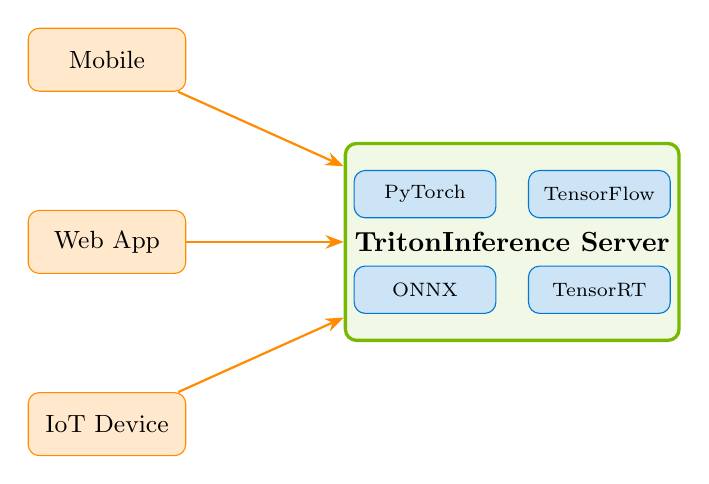
\begin{tikzpicture}[
    node distance=0.8cm and 1.2cm,
    server/.style={rectangle, rounded corners, minimum width=4cm, minimum height=2.5cm, draw=nvidiagreen, fill=nvidiagreen!10, very thick, font=\bfseries},
    model/.style={rectangle, rounded corners, minimum width=1.8cm, minimum height=0.6cm, draw=nvidiablue, fill=nvidiablue!20, font=\scriptsize},
    client/.style={rectangle, rounded corners, minimum width=2cm, minimum height=0.8cm, draw=accentorange, fill=accentorange!20, font=\small},
    arrow/.style={-Stealth, thick}
]

% Triton Server
\node[server] (triton) at (0,0) {Triton\\Inference Server};

% Models inside server
\node[model, above left=0.3cm and 0.2cm of triton.center] (pytorch) {PyTorch};
\node[model, above right=0.3cm and 0.2cm of triton.center] (tf) {TensorFlow};
\node[model, below left=0.3cm and 0.2cm of triton.center] (onnx) {ONNX};
\node[model, below right=0.3cm and 0.2cm of triton.center] (trt) {TensorRT};

% Client applications
\node[client, left=2cm of triton] (web) {Web App};
\node[client, above=1.5cm of web] (mobile) {Mobile};
\node[client, below=1.5cm of web] (iot) {IoT Device};

% Arrows
\draw[arrow, accentorange] (web) -- (triton);
\draw[arrow, accentorange] (mobile) -- (triton);
\draw[arrow, accentorange] (iot) -- (triton);

\end{tikzpicture}
\caption{Triton Inference Server Architecture}
\label{fig:triton}
\end{figure}

\textbf{Triton Key Capabilities:}
\begin{itemize}[leftmargin=*, itemsep=5pt]
    \item \textbf{Multi-framework Support:} TensorFlow, PyTorch, ONNX, TensorRT, and custom backends
    \item \textbf{Dynamic Batching:} Automatically combines requests for optimal throughput
    \item \textbf{Model Ensemble:} Chain multiple models in inference pipelines
    \item \textbf{Concurrent Execution:} Run multiple model instances simultaneously
    \item \textbf{GPU/CPU Flexibility:} Deploy on heterogeneous infrastructure
\end{itemize}

\section{Layer 6: Software Distribution}

\subsection{NGC Catalog}

The NVIDIA GPU Cloud (NGC) catalog serves as a comprehensive repository of GPU-optimized software, including pre-trained models, containers, and SDKs.

\begin{keypoint}
NGC provides verified, tested, and optimized resources that accelerate AI development from prototyping to production deployment.
\end{keypoint}

\textbf{NGC Resources:}
\begin{itemize}[leftmargin=*, itemsep=5pt]
    \item \textbf{Containers:} Pre-configured Docker images with optimized frameworks
    \item \textbf{Pre-trained Models:} Ready-to-use models for common tasks
    \item \textbf{Helm Charts:} Kubernetes deployment configurations
    \item \textbf{SDKs and Libraries:} Development toolkits and APIs
    \item \textbf{Industry Solutions:} Domain-specific applications and workflows
\end{itemize}

% ==================== CHAPTER 3: DEPLOYMENT ====================
\chapter{Deployment Options and Integration}

\section{Deployment Strategies}

\begin{table}[H]
\centering
\caption{NVIDIA Stack Deployment Options}
\begin{tabularx}{\textwidth}{l X X}
\toprule
\textcolor{nvidiagreen}{\textbf{Option}} & \textcolor{nvidiagreen}{\textbf{Advantages}} & \textcolor{nvidiagreen}{\textbf{Use Cases}} \\
\midrule
On-Premises & Full control, data privacy, customization & Regulated industries, sensitive data \\
Public Cloud & Scalability, pay-as-you-go, managed services & Variable workloads, experimentation \\
Hybrid & Best of both worlds, workload optimization & Enterprise with mixed requirements \\
Edge & Low latency, offline capability & IoT, autonomous systems, retail \\
\bottomrule
\end{tabularx}
\label{tab:deployment}
\end{table}

\subsection{On-Premises Deployment}

For organizations requiring maximum control over their AI infrastructure, NVIDIA provides comprehensive reference architectures and partner support.

\textbf{Self-Deployment Considerations:}
\begin{enumerate}[leftmargin=*, itemsep=5pt]
    \item \textbf{Hardware Selection:} Choose appropriate GPU models based on workload
    \item \textbf{Networking:} Design high-bandwidth interconnects for multi-GPU systems
    \item \textbf{Cooling and Power:} Plan for significant power and cooling requirements
    \item \textbf{Software Stack:} Install and configure CUDA, drivers, and frameworks
    \item \textbf{Monitoring:} Implement GPU utilization and performance tracking
\end{enumerate}

\subsection{Cloud Deployment}

Major cloud providers offer NVIDIA GPU instances with pre-configured software stacks:

\begin{nvidiabox}[Cloud Provider Options]
\begin{itemize}[leftmargin=*, itemsep=5pt]
    \item \textbf{AWS:} EC2 P4/P5 instances, SageMaker with NVIDIA GPU support
    \item \textbf{Microsoft Azure:} NC/ND-series VMs, Azure Machine Learning
    \item \textbf{Google Cloud:} A2/A3 instances, Vertex AI with GPU acceleration
    \item \textbf{Oracle Cloud:} GPU instances with flexible configurations
\end{itemize}
\end{nvidiabox}

\section{Third-Party Integrations}

\subsection{Container Orchestration}

\begin{figure}[H]
\centering
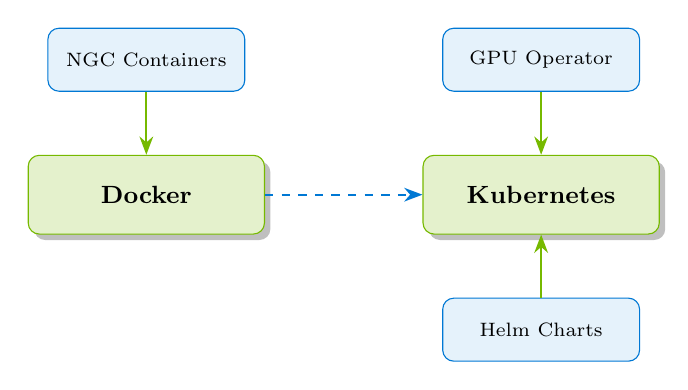
\begin{tikzpicture}[
    node distance=1.2cm,
    component/.style={rectangle, rounded corners, minimum width=3cm, minimum height=1cm, text centered, draw=nvidiagreen, fill=nvidiagreen!20, font=\small\bfseries, drop shadow},
    integration/.style={rectangle, rounded corners, minimum width=2.5cm, minimum height=0.8cm, text centered, draw=nvidiablue, fill=nvidiablue!10, font=\scriptsize},
    arrow/.style={-Stealth, thick, color=nvidiagreen}
]

\node[component] (docker) {Docker};
\node[component, right=2cm of docker] (k8s) {Kubernetes};
\node[integration, above=0.8cm of docker] (ngc1) {NGC Containers};
\node[integration, above=0.8cm of k8s] (ngc2) {GPU Operator};
\node[integration, below=0.8cm of k8s] (helm) {Helm Charts};

\draw[arrow] (ngc1) -- (docker);
\draw[arrow] (ngc2) -- (k8s);
\draw[arrow] (helm) -- (k8s);
\draw[arrow, dashed, nvidiablue] (docker) -- (k8s);

\end{tikzpicture}
\caption{Container Orchestration Integration}
\label{fig:containers}
\end{figure}

\textbf{Docker Integration:}
\begin{itemize}[leftmargin=*, itemsep=5pt]
    \item NVIDIA Container Toolkit for GPU access within containers
    \item Pre-built NGC containers with optimized frameworks
    \item Multi-GPU container support
\end{itemize}

\textbf{Kubernetes Integration:}
\begin{itemize}[leftmargin=*, itemsep=5pt]
    \item NVIDIA GPU Operator for automated GPU driver and runtime management
    \item GPU scheduling and resource allocation
    \item Multi-instance GPU (MIG) support for resource sharing
\end{itemize}

\subsection{Machine Learning Frameworks}

NVIDIA maintains deep integration with leading ML frameworks:

\begin{table}[H]
\centering
\caption{Framework Integration Features}
\begin{tabularx}{\textwidth}{l X}
\toprule
\textcolor{nvidiagreen}{\textbf{Framework}} & \textcolor{nvidiagreen}{\textbf{NVIDIA Integration}} \\
\midrule
PyTorch & CUDA acceleration, cuDNN integration, Apex (mixed precision) \\
TensorFlow & GPU-optimized operations, XLA compiler, TensorRT integration \\
JAX & GPU/TPU acceleration, XLA compilation \\
ONNX & TensorRT conversion, optimization tools \\
\bottomrule
\end{tabularx}
\label{tab:frameworks}
\end{table}

\subsection{Workflow Automation}

Integration with orchestration and workflow tools enables complex AI pipelines:

\begin{itemize}[leftmargin=*, itemsep=5pt]
    \item \textbf{LangChain:} Building LLM-powered applications with GPU acceleration
    \item \textbf{Apache Airflow:} Orchestrating GPU-accelerated data pipelines
    \item \textbf{Kubeflow:} End-to-end ML workflows on Kubernetes with GPU support
    \item \textbf{MLflow:} Experiment tracking and model management with GPU metrics
\end{itemize}

% ==================== CHAPTER 4: BEST PRACTICES ====================
\chapter{Best Practices and Optimization}

\section{GPU Utilization Optimization}

\begin{nvidiabox}[Maximizing GPU Efficiency]
Proper GPU utilization is critical for achieving optimal performance and cost-effectiveness in AI workloads.
\end{nvidiabox}

\subsection{Performance Optimization Strategies}

\begin{enumerate}[leftmargin=*, itemsep=8pt]
    \item \textbf{Batch Size Optimization}
    \begin{itemize}
        \item Larger batches improve GPU utilization
        \item Balance between throughput and memory constraints
        \item Dynamic batching for inference workloads
    \end{itemize}
    
    \item \textbf{Mixed Precision Training}
    \begin{itemize}
        \item FP16/BF16 for faster computation with maintained accuracy
        \item Automatic mixed precision (AMP) frameworks
        \item Gradient scaling to prevent underflow
    \end{itemize}
    
    \item \textbf{Data Pipeline Optimization}
    \begin{itemize}
        \item Prefetching to hide data loading latency
        \item GPU-direct data loading when possible
        \item Parallel data preprocessing
    \end{itemize}
    
    \item \textbf{Model Parallelism}
    \begin{itemize}
        \item Tensor parallelism for large models
        \item Pipeline parallelism for deep networks
        \item Hybrid strategies combining multiple approaches
    \end{itemize}
\end{enumerate}

\section{Cost Optimization}

\begin{table}[H]
\centering
\caption{Cost Optimization Techniques}
\begin{tabularx}{\textwidth}{l X l}
\toprule
\textcolor{nvidiagreen}{\textbf{Technique}} & \textcolor{nvidiagreen}{\textbf{Description}} & \textcolor{nvidiagreen}{\textbf{Savings}} \\
\midrule
Spot Instances & Use preemptible cloud instances for training & 60-90\% \\
Model Quantization & Reduce precision for inference & 4-8x \\
Multi-Instance GPU & Share single GPU across workloads & 2-7x \\
Auto-scaling & Dynamic resource allocation & 30-50\% \\
Checkpoint Resume & Resume interrupted training & Variable \\
\bottomrule
\end{tabularx}
\label{tab:cost-opt}
\end{table}

% ==================== CHAPTER 5: ECOSYSTEM DIAGRAM ====================
\chapter{Complete Ecosystem Visualization}

\section{End-to-End AI Workflow}

\begin{figure}[H]
\centering
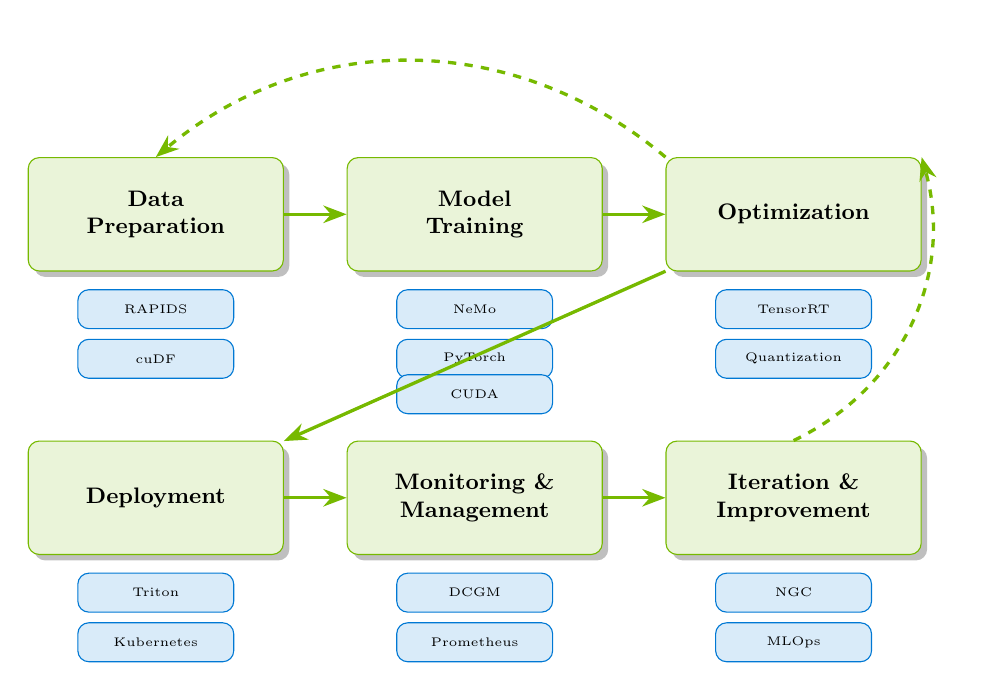
\begin{tikzpicture}[
    scale=0.9,
    every node/.style={transform shape},
    phase/.style={
        rectangle, rounded corners,
        minimum width=3.6cm, minimum height=1.6cm,
        text centered, text width=3.2cm,
        draw=nvidiagreen, fill=nvidiagreen!15,
        font=\small\bfseries, drop shadow
    },
    tool/.style={
        rectangle, rounded corners,
        minimum width=2.2cm, minimum height=0.55cm,
        text centered,
        draw=nvidiablue, fill=nvidiablue!15,
        font=\tiny
    },
    arrow/.style={-Stealth, very thick, color=nvidiagreen}
]

% --- phases in a regular grid ---
\node[phase] (data)        at (0,0)   {Data\\Preparation};
\node[phase] (training)    at (4.5,0) {Model\\Training};
\node[phase] (optimization)at (9,0)   {Optimization};

\node[phase] (deployment)  at (0,-4)  {Deployment};
\node[phase] (monitoring)  at (4.5,-4){Monitoring \&\\Management};
\node[phase] (iteration)   at (9,-4)  {Iteration \&\\Improvement};

% --- tools under each phase (no overlaps) ---
\node[tool, below=0.25cm of data]      {RAPIDS};
\node[tool, below=0.95cm of data]      {cuDF};

\node[tool, below=0.25cm of training]  {NeMo};
\node[tool, below=0.95cm of training]  {PyTorch};
\node[tool, below=1.45cm of training]  {CUDA};

\node[tool, below=0.25cm of optimization] {TensorRT};
\node[tool, below=0.95cm of optimization] {Quantization};

\node[tool, below=0.25cm of deployment] {Triton};
\node[tool, below=0.95cm of deployment] {Kubernetes};

\node[tool, below=0.25cm of monitoring] {DCGM};
\node[tool, below=0.95cm of monitoring] {Prometheus};

\node[tool, below=0.25cm of iteration]  {NGC};
\node[tool, below=0.95cm of iteration]  {MLOps};

% --- arrows between phase boxes only ---
\draw[arrow] (data) -- (training);
\draw[arrow] (training) -- (optimization);
\draw[arrow] (optimization) -- (deployment);
\draw[arrow] (deployment) -- (monitoring);
\draw[arrow] (monitoring) -- (iteration);
\draw[arrow, dashed, bend right=40] (iteration.north) to (optimization.north east);
\draw[arrow, dashed, bend right=40] (optimization.north west) to (data.north);

\end{tikzpicture}
\caption{Complete NVIDIA AI Workflow with Ecosystem Tools}
\label{fig:workflow}
\end{figure}


\newpage
\section{Comprehensive Stack Diagram}

\begin{figure}[H]
\centering
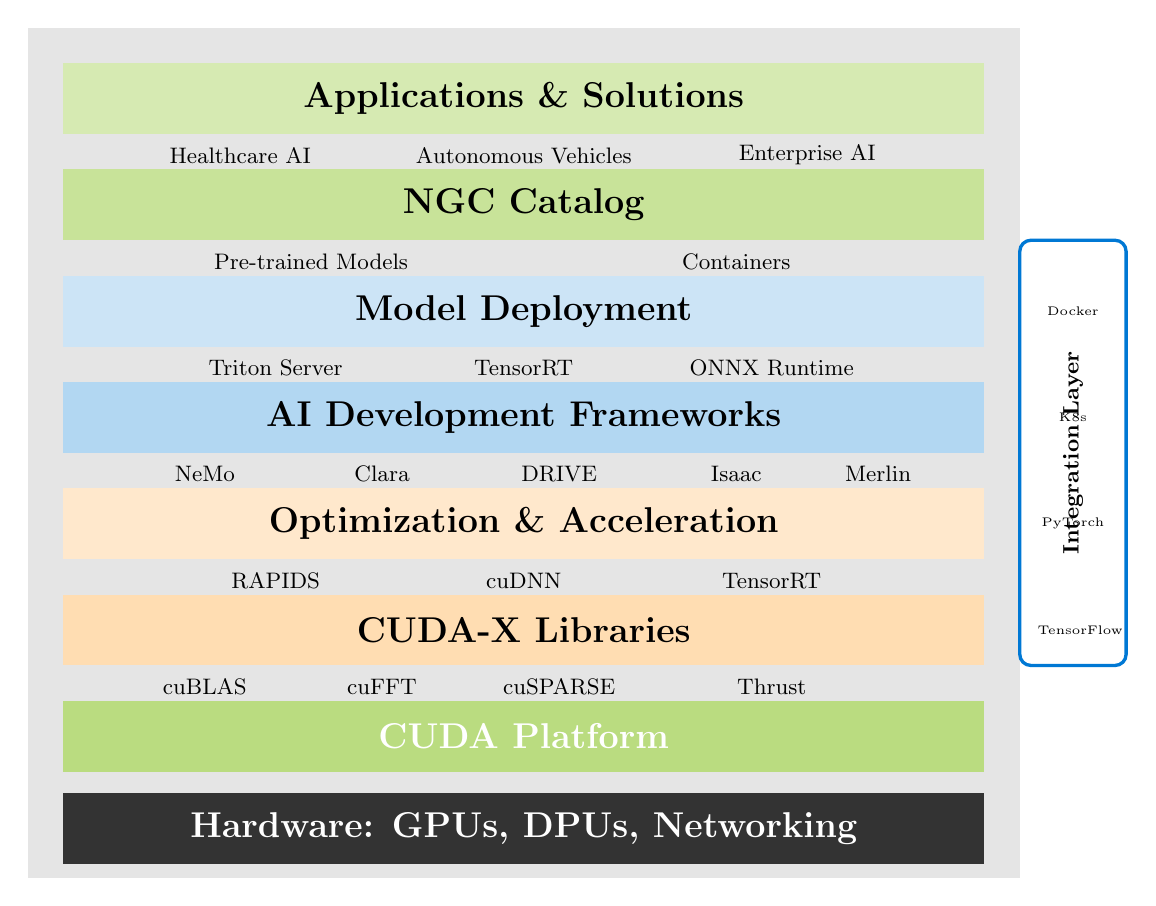
\begin{tikzpicture}[
    scale=0.9,
    every node/.style={transform shape}
]

% Background layers
\fill[nvidiablack!10] (0,0) rectangle (14,12);

% Layer 6 - Applications
\fill[nvidiagreen!30] (0.5,10.5) rectangle (13.5,11.5);
\node[font=\Large\bfseries] at (7,11) {Applications \& Solutions};
\node[font=\small] at (3,10.2) {Healthcare AI};
\node[font=\small] at (7,10.2) {Autonomous Vehicles};
\node[font=\small] at (11,10.2) {Enterprise AI};

% Layer 5 - NGC
\fill[nvidiagreen!40] (0.5,9) rectangle (13.5,10);
\node[font=\Large\bfseries] at (7,9.5) {NGC Catalog};
\node[font=\small] at (4,8.7) {Pre-trained Models};
\node[font=\small] at (10,8.7) {Containers};

% Layer 4 - Deployment
\fill[nvidiablue!20] (0.5,7.5) rectangle (13.5,8.5);
\node[font=\Large\bfseries] at (7,8) {Model Deployment};
\node[font=\small] at (3.5,7.2) {Triton Server};
\node[font=\small] at (7,7.2) {TensorRT};
\node[font=\small] at (10.5,7.2) {ONNX Runtime};

% Layer 3 - Frameworks
\fill[nvidiablue!30] (0.5,6) rectangle (13.5,7);
\node[font=\Large\bfseries] at (7,6.5) {AI Development Frameworks};
\node[font=\small] at (2.5,5.7) {NeMo};
\node[font=\small] at (5,5.7) {Clara};
\node[font=\small] at (7.5,5.7) {DRIVE};
\node[font=\small] at (10,5.7) {Isaac};
\node[font=\small] at (12,5.7) {Merlin};

% Layer 2 - Optimization
\fill[accentorange!20] (0.5,4.5) rectangle (13.5,5.5);
\node[font=\Large\bfseries] at (7,5) {Optimization \& Acceleration};
\node[font=\small] at (3.5,4.2) {RAPIDS};
\node[font=\small] at (7,4.2) {cuDNN};
\node[font=\small] at (10.5,4.2) {TensorRT};

% Layer 1 - Libraries
\fill[accentorange!30] (0.5,3) rectangle (13.5,4);
\node[font=\Large\bfseries] at (7,3.5) {CUDA-X Libraries};
\node[font=\small] at (2.5,2.7) {cuBLAS};
\node[font=\small] at (5,2.7) {cuFFT};
\node[font=\small] at (7.5,2.7) {cuSPARSE};
\node[font=\small] at (10.5,2.7) {Thrust};

% Layer 0 - CUDA
\fill[nvidiagreen!50] (0.5,1.5) rectangle (13.5,2.5);
\node[font=\Large\bfseries\color{nvidiawhite}] at (7,2) {CUDA Platform};

% Hardware Foundation
\fill[nvidiablack!80] (0.5,0.2) rectangle (13.5,1.2);
\node[font=\Large\bfseries\color{nvidiawhite}] at (7,0.7) {Hardware: GPUs, DPUs, Networking};

% Integration boxes on sides
\draw[nvidiablue, very thick, rounded corners] (14,3) rectangle (15.5,9);
\node[rotate=90, font=\small\bfseries] at (14.75,6) {Integration Layer};
\node[font=\tiny, text width=1cm, align=center] at (14.75,8) {Docker};
\node[font=\tiny, text width=1cm, align=center] at (14.75,6.5) {K8s};
\node[font=\tiny, text width=1cm, align=center] at (14.75,5) {PyTorch};
\node[font=\tiny, text width=1cm, align=center] at (14.75,3.5) {TensorFlow};

\end{tikzpicture}
\caption{Complete NVIDIA Software Stack Architecture}
\label{fig:complete-stack}
\end{figure}

% ==================== CHAPTER 6: CASE STUDIES ====================
\chapter{Real-World Applications}

\section{Use Case: Large Language Model Training}

\begin{nvidiabox}[LLM Training Scenario]
Training a 70B parameter language model using NVIDIA infrastructure and software stack.
\end{nvidiabox}

\subsection{Architecture Overview}

\begin{table}[H]
\centering
\caption{LLM Training Infrastructure}
\begin{tabularx}{\textwidth}{l X}
\toprule
\textcolor{nvidiagreen}{\textbf{Component}} & \textcolor{nvidiagreen}{\textbf{Specification}} \\
\midrule
Hardware & 32x NVIDIA A100 80GB GPUs (4 DGX nodes) \\
Networking & 8x 200Gbps InfiniBand per node \\
Framework & NeMo with Megatron-LM \\
Parallelism & 3D parallelism (tensor + pipeline + data) \\
Optimization & Mixed precision (BF16), gradient checkpointing \\
Storage & Parallel filesystem (Lustre) for checkpoints \\
\bottomrule
\end{tabularx}
\label{tab:llm-infra}
\end{table}

\subsection{Performance Metrics}

\begin{itemize}[leftmargin=*, itemsep=5pt]
    \item \textbf{Training Throughput:} 140 TFLOPS per GPU sustained
    \item \textbf{Time to Train:} 2-3 weeks for complete training run
    \item \textbf{GPU Utilization:} 85-92\% average utilization
    \item \textbf{Model Quality:} Comparable to state-of-the-art benchmarks
\end{itemize}

\section{Use Case: Healthcare Imaging Analysis}

Using NVIDIA Clara for medical image segmentation and diagnosis support.

\begin{keypoint}
Clara's pre-trained models and GPU acceleration reduced medical image analysis time from hours to seconds, enabling real-time clinical decision support.
\end{keypoint}

\textbf{Implementation Details:}
\begin{itemize}[leftmargin=*, itemsep=5pt]
    \item Clara imaging SDK for DICOM processing
    \item Pre-trained segmentation models from NGC
    \item TensorRT optimization for sub-second inference
    \item Triton deployment for hospital PACS integration
    \item HIPAA-compliant on-premises deployment
\end{itemize}

% ==================== CHAPTER 7: FUTURE DIRECTIONS ====================
\chapter{Future of NVIDIA Ecosystem}

\section{Emerging Technologies}

\begin{table}[H]
\centering
\caption{NVIDIA Future Technology Roadmap}
\begin{tabularx}{\textwidth}{l l X}
\toprule
\textcolor{nvidiagreen}{\textbf{Technology}} & \textcolor{nvidiagreen}{\textbf{Timeline}} & \textcolor{nvidiagreen}{\textbf{Impact}} \\
\midrule
Grace Hopper & 2024-2025 & Unified CPU-GPU architecture for AI \\
Blackwell & 2024-2025 & Next-gen GPU with 4x AI performance \\
Quantum-2 & 2025+ & 400Gbps InfiniBand networking \\
NVLink 5.0 & 2025+ & Higher GPU-to-GPU bandwidth \\
Generative AI & Ongoing & Foundation models and tools \\
\bottomrule
\end{tabularx}
\label{tab:future}
\end{table}

\section{Industry Trends}

\subsection{Democratization of AI}

NVIDIA is working to make AI accessible to organizations of all sizes through:
\begin{itemize}[leftmargin=*, itemsep=5pt]
    \item Cloud-based GPU access reducing capital expenses
    \item Pre-trained models eliminating training requirements
    \item AutoML tools simplifying model development
    \item Edge AI bringing intelligence closer to data sources
\end{itemize}

\subsection{Sustainable AI}

Energy efficiency and sustainability initiatives:
\begin{itemize}[leftmargin=*, itemsep=5pt]
    \item More efficient GPU architectures (performance per watt)
    \item Dynamic power management and scheduling
    \item Liquid cooling solutions for data centers
    \item Carbon-aware workload scheduling
\end{itemize}

% ==================== APPENDIX ====================
\appendix

\chapter{Quick Reference}

\section{Command Reference}

\begin{lstlisting}[language=bash, caption=Essential NVIDIA Commands]
# Check GPU availability
nvidia-smi

# Monitor GPU utilization
watch -n 1 nvidia-smi

# Run container with GPU support
docker run --gpus all nvidia/cuda:12.3-base

# Check CUDA version
nvcc --version

# Profile GPU application
nsys profile -o output ./application
\end{lstlisting}

\section{Common Configurations}

\begin{lstlisting}[language=Python, caption=PyTorch GPU Configuration]
import torch

# Check GPU availability
device = torch.device("cuda" if torch.cuda.is_available() else "cpu")
print(f"Using device: {device}")

# Enable mixed precision training
from torch.cuda.amp import autocast, GradScaler
scaler = GradScaler()

# Model parallelism
model = torch.nn.DataParallel(model)
\end{lstlisting}

\section{Resource Links}

\begin{table}[H]
\centering
\caption{Essential NVIDIA Resources}
\begin{tabularx}{\textwidth}{l X}
\toprule
\textcolor{nvidiagreen}{\textbf{Resource}} & \textcolor{nvidiagreen}{\textbf{URL}} \\
\midrule
NGC Catalog & \url{https://catalog.ngc.nvidia.com} \\
Developer Documentation & \url{https://docs.nvidia.com} \\
CUDA Toolkit & \url{https://developer.nvidia.com/cuda-toolkit} \\
Deep Learning SDK & \url{https://developer.nvidia.com/deep-learning} \\
Forums & \url{https://forums.developer.nvidia.com} \\
GitHub & \url{https://github.com/NVIDIA} \\
\bottomrule
\end{tabularx}
\label{tab:resources}
\end{table}

% ==================== GLOSSARY ====================
\chapter{Glossary}

\begin{description}[style=nextline, leftmargin=2cm, font=\bfseries\color{nvidiagreen}]
    \item[CUDA] Compute Unified Device Architecture - parallel computing platform and API
    \item[cuDNN] CUDA Deep Neural Network library for deep learning primitives
    \item[DGX] NVIDIA's integrated AI systems combining GPUs and optimized software
    \item[GPU] Graphics Processing Unit - specialized processor for parallel computations
    \item[InfiniBand] High-performance networking technology for HPC and AI clusters
    \item[NGC] NVIDIA GPU Cloud - catalog of GPU-optimized software
    \item[NeMo] NVIDIA framework for conversational AI model development
    \item[RAPIDS] Suite of open-source libraries for GPU-accelerated data science
    \item[Tensor Core] Specialized hardware units for matrix operations in AI workloads
    \item[TensorRT] SDK for high-performance deep learning inference
    \item[Triton] Inference server for deploying AI models at scale
\end{description}

% ==================== BIBLIOGRAPHY ====================
\begin{thebibliography}{99}

\bibitem{nvidia_arch}
NVIDIA Corporation. (2024). \textit{NVIDIA GPU Architecture Documentation}.
\url{https://docs.nvidia.com/cuda/}

\bibitem{cuda_guide}
NVIDIA Corporation. (2024). \textit{CUDA C Programming Guide}.
\url{https://docs.nvidia.com/cuda/cuda-c-programming-guide/}

\bibitem{nemo_docs}
NVIDIA Corporation. (2024). \textit{NeMo Framework Documentation}.
\url{https://docs.nvidia.com/deeplearning/nemo/}

\bibitem{triton_docs}
NVIDIA Corporation. (2024). \textit{Triton Inference Server Documentation}.
\url{https://docs.nvidia.com/deeplearning/triton-inference-server/}

\bibitem{rapids_docs}
NVIDIA Corporation. (2024). \textit{RAPIDS AI Documentation}.
\url{https://rapids.ai/}

\bibitem{tensorrt_docs}
NVIDIA Corporation. (2024). \textit{TensorRT Developer Guide}.
\url{https://docs.nvidia.com/deeplearning/tensorrt/}

\end{thebibliography}

% ==================== BACK COVER ====================

\newpage
\thispagestyle{empty}
\begin{tikzpicture}[remember picture,overlay]
    \fill[nvidiablack] (current page.south west) rectangle (current page.north east);
    
    \fill[nvidiagreen] (current page.north west) rectangle ([yshift=-3cm]current page.north east);
    \fill[nvidiagreen] ([yshift=3cm]current page.south west) rectangle (current page.south east);
    
    \node[text=nvidiawhite,font=\fontsize{32}{40}\selectfont\bfseries,text width=10cm,align=center] at (current page.center) 
    {NVIDIA Ecosystem\\[0.5cm]};
    
    \node[text=nvidialightgray,font=\fontsize{14}{18}\selectfont,text width=12cm,align=center] at ([yshift=-3cm]current page.center) 
    {From hardware to software, from training to deployment\\[0.5cm]
    This comprehensive guide covers the complete NVIDIA AI stack\\[0.3cm]
    
    \href{https://github.com/Yash-Kavaiya/awesome-nvidia}{awesome-nvidia} | \href{https://github.com/Yash-Kavaiya/NvDev}{NvDev}};
    
    \node[text=nvidiagreen,font=\fontsize{16}{20}\selectfont\bfseries] at ([yshift=-6cm]current page.center) 
    {\href{https://easy-ai-labs.lovable.app/}{Easy AI Labs} | \href{https://www.linkedin.com/in/yashkavaiya}{Yash Kavaiya} | \href{https://www.linkedin.com/company/genai-guru}{Gen AI Guru}};
\end{tikzpicture}

\end{document}
